\section{Security Model}
\subsection{Taxonomy of Timing Channels}
    \begin{figure}
        \begin{center}
            \includegraphics[width=2.2in]{figs/taxonomy.pdf}
            \caption{The taxonomy of timing channels}
            \label{fig:taxonomy}
        \end{center}
    \end{figure}

A timing channel is a vulnerability that correlates secret data with the  
timing of events within a system thereby forming a channel for communicating or 
extracting secret data despite the intentions of the system designer. Figure 
\ref{fig:taxonomy} summarizes the taxonomy of timing channels. \emph{Direct} or 
language level timing channels can be identified by examining the source code 
\cite{mitigation3}. A password checking algorithm that stops as soon as an 
incorrect character is found causes a direct timing channel that leaks 
information about the correct password. In contrast, \emph{indirect} or 
microarchitectural timing channels cannot be identified in the source code 
since they depend on hardware level behavior \cite{mitigation3}. Conventional 
caches cause an indirect timing channel whenever the probability of a cache hit 
depends on secret data. Programming language techniques have been developed to 
address language level timing channels 
\cite{timesens,mitigation1,mitigation2,mitigation3}. It is possible to reduce 
the information leaked by some microarchitectural timing channels at the 
language level \cite{mitigation3}. However, eliminating all leakage caused by 
microarchitectural timing channels is difficult without hardware support.
%%%% More precise, wordier version:
%  However, efficiently providing strict timing-sensitive noninterference in 
%  the presence microarchitectural timing channels without the support of 
%  hardware is a hard problem.

Microarchitectural timing channels can be further divided into internal or 
external timing channels. \emph{External} timing channels are not caused by 
interference, and are exploited by an adversary that directly measures the 
timing of the victim's actions. External timing channels can be exploited by an 
adversary that does not share hardware with the victim. Bernstein's 
attack~\cite{bernstein} exploits an external timing channel in popular 
implementations of AES (such as OpenSSL). The external timing channel exists 
because the cache access pattern both affects the overall execution time of the 
AES implementation and depends on the secret key. The adversary carries out the 
attack without sharing any hardware by directly measuring the response times of 
the victim machine.
% The long explanation
% The adversary uses a copy of the same AES implementation as the victim to 
% time the encryption of a number inputs with a known key on the adversary's 
% local machine. Then, the adversary makes requests to the victim machine using 
% the same inputs and times how long the victim machine takes to encrypt the 
% inputs with an unknown key. In both cases, the execution time depends on the 
% cache access pattern which depends on the key. The adversary can use the 
% timing information gathered with the known and unknown keys to learn the 
% secret AES key.

\emph{Internal} timing channels are exploited by an adversary that shares 
hardware with the victim, and are caused by interference between the adversary 
and the victim. An adversary exploits the internal timing channel by measuring 
the timing of its own actions rather than measuring the actions of the victim 
directly. Percival~\cite{percival} has shown that the an internal timing 
channel through the cache. The attacker shares hardware with a victim process 
running a vulnerable implementation of AES. The attacker extracts information 
by measuring it's own cache access times to observe the victim's interference 
which correlates to the secret key.

Internal microarchitectural timing channels can either be state based, or 
contention based. In a \emph{state based} timing channel, the victim and 
adversary share some hardware state element with access timing that depends on 
its contents. Conventional shared caches have state based timing channels; 
accesses to memory addresses in the cache are faster than those that are not.
In a \emph{contention based} timing channel, the victim and adversary share a 
resource that can handle only a finite number of requests at a time.  Requests 
made to the resource while it is already handling a request are delayed. 
Conventional buses have contention based timing channels since a finite number 
of requests can be transferred at a time while the remaining requests are 
delayed in a queue.

%% Not sure if the covert channel paragraph is needed
We show how this taxonomy can be used to identify general approaches to prevent 
each type of timing channel in Section \ref{sec:tc_sources}. Though the use of 
a victim and an adversary in these definitions may seem to limit this taxonomy 
to timing side channels, it is equally valid for categorizing timing covert 
channels. To categorize covert channels, the victim is replaced with an 
adversary that intentionally sends messages to a second adversary through the 
timing channel.

\subsection{Threat Model}
%Goal
The goal of this work is to completely isolate distrusting software entities, 
such as threads, processes, or virtual machines that share hardware. The system 
should be no less secure than running the software entities on separate 
hardware. 

%Assumptions
The multicore system of interest consists of hardware resources that are
concurrently shared by multiple software entities. It is possible for software 
entities to be time multiplexed on the same core (e.g.  by context switching 
VMs), but the system does not allow software entities to execute concurrently 
on the same core (e.g. through simultaneous multithreading). 
We assume that a trusted software layer, such as an OS, uses conventional 
software isolation abstractions such as threads, processes, and machine 
virtualization. Along with access controls, these provide isolation through 
explicit channels.

%Attacks we handle.
However, these approaches to isolate software do not address timing channels 
that leverage shared hardware. To guarantee total isolation, internal timing 
channels must also be eliminated. We eliminate all internal microarchitectural 
timing channels including state and state-based timing channels. This includes 
all timing channels caused by concurrently shared resources as well as timing 
channels in hardware that is shared through time multiplexing (e.g. by context 
switching).

%Attacks we don't handle.
Since our goal is to address vulnerabilities 
caused by hardware sharing,
timing channels that are external to the hardware are not addressed.
Any timing channels that are external to the hardware in this system would also 
be present if the software entities executed on separate hardware. If 
necessary, external timing channels can be controlled in software. Similarly, 
we do not address language level timing channels since these may also be 
addressed in software.  Lastly, we do not consider physical attacks and assume 
that the adversary does not have physical access.
